% genesis_mnras.tex
%
% GENESIS — MNRAS Manuscript
% Based on mnras_template.tex v3.3 (April 2024)
%
% FILL MARKERS:  \FILL{description}  — replace with actual values
% TODO MARKERS:  % TODO: ...         — action items before submission
%
% Compile:  pdflatex genesis_mnras.tex
%           bibtex   genesis_mnras
%           pdflatex genesis_mnras.tex (x2)

%%%%%%%%%%%%%%%%%%%%%%%%%%%%%%%%%%%%%%%%%%%%%%%%%%
\documentclass[usenatbib]{mnras}

% \usepackage{newtxtext,newtxmath}  % preferred; uncomment if available
\usepackage{mathptmx}  % fallback Times font
\usepackage[T1]{fontenc}

\DeclareRobustCommand{\VAN}[3]{#2}
\let\VANthebibliography\thebibliography
\def\thebibliography{\DeclareRobustCommand{\VAN}[3]{##3}\VANthebibliography}

%%%%% EXTRA PACKAGES %%%%%
\usepackage{graphicx}
\usepackage{amsmath}
\usepackage{amssymb}
\usepackage{booktabs}
\usepackage{xcolor}
\usepackage{hyperref}
\usepackage{microtype}
\usepackage{multirow}
\usepackage{siunitx}
\usepackage{enumitem}

%%%%% CUSTOM COMMANDS %%%%%
\newcommand{\FILL}[1]{\textcolor{red}{\textbf{[#1]}}}
\newcommand{\Mcdm}{M_{\rm cdm}}
\newcommand{\Mgas}{M_{\rm gas}}
\newcommand{\Tgas}{T}
\newcommand{\Om}{\Omega_{\rm m}}
\newcommand{\sig}{\sigma_8}
\newcommand{\thetavec}{\boldsymbol{\theta}}
\newcommand{\kvec}{\boldsymbol{k}}
\newcommand{\Pk}{P(k)}
\newcommand{\Pkab}{P_{ab}(k)}
\newcommand{\rab}{r_{ab}(k)}
\newcommand{\DeltaP}{\Delta P/P}

%%%%%%%%%%%%%%%%%%% TITLE PAGE %%%%%%%%%%%%%%%%%%%

\title[GENESIS: Cosmological Structure Emulation]{%
GENESIS: Generative Emulator Networks for Inference and Simulation of
Cosmological Structure}

\author[M. Park]{%
Minje Park$^{1}$\thanks{E-mail: pmj0324@g.skku.edu}
\\
$^{1}$Department of Physics, Sungkyunkwan University, Suwon 16419, Republic of Korea
}

\date{Accepted XXX. Received YYY; in original form ZZZ}

\pubyear{\the\year{}}

%%%%%%%%%%%%%%%%%%%%%%%%%%%%%%%%%%%%%%%%%%%%%%%%%%

\begin{document}
\label{firstpage}
\pagerange{\pageref{firstpage}--\pageref{lastpage}}
\maketitle

%% ── Abstract ──────────────────────────────────────────────────────────────
\begin{abstract}
Machine-learning methods in cosmology increasingly rely on large,
physically realistic training sets drawn from hydrodynamic simulations,
but the cost of such simulations limits dense coverage of cosmological
and astrophysical parameter space.
The CAMELS project and its public CAMELS Multifield Dataset provide a
controlled setting for learning from multiple correlated fields across
this design space, yet existing approaches have focused primarily on
single-field generation or have validated multifield outputs through
per-channel summaries alone.
We present \textsc{Genesis}, a conditional generative model that
produces dark matter density, gas density, and gas temperature fields
as a correlated triplet, conditioned on all six CAMELS parameters
including four astrophysical feedback parameters.
The model uses optimal-transport flow matching (OT-FM) with a U-Net backbone
incorporating periodic-boundary convolutions and channel
squeeze-and-excitation.
We evaluate \textsc{Genesis} as a field-level multifield emulator on
$256^2$ maps at $25\,h^{-1}$~Mpc, using auto-power spectra,
cross-power spectra, inter-field coherence, one-point distributions,
cosmic-variance consistency, and parameter-response tests across four
CAMELS validation protocols (LH, CV, 1P, EX).
The model reproduces key per-field and cross-field statistics of the
target simulations across a broad range of scales, suggesting that
OT-FM-based multifield emulators offer a practical path toward
fast cosmological forward modelling.
\end{abstract}

\begin{keywords}
methods: numerical -- methods: statistical --
cosmology: large-scale structure of Universe -- galaxies: formation
\end{keywords}

%%%%%%%%%%%%%%%%%%%%%%%%%%%%%%%%%%%%%%%%%%%%%%%%%%

%%%%%%%%%%%%%%%%% BODY OF PAPER %%%%%%%%%%%%%%%%%%

%% =============================================================
%%  §1  INTRODUCTION
%% =============================================================
\section{Introduction}
\label{sec:intro}

In modern cosmology, machine learning has emerged as an indispensable
tool across a broad range of inference and modelling problems,
including cosmological parameter inference
\citep{Ravanbakhsh2017,Cranmer2020}, field-level analyses and baryonic
field mapping \citep{JoKim2019,Zhang2019}, generative modelling of
cosmological fields \citep{Mustafa2019}, and the emulation of
expensive simulations \citep{He2019,Perraudin2021}.
As in many other machine-learning settings, progress in these problems
depends on access to large and diverse training sets. In cosmology,
such training sets are often provided by large suites of hydrodynamic
simulations that span both cosmological and astrophysical parameter
space, but these simulation campaigns remain computationally expensive.
The Cosmology and Astrophysics with Machine Learning Simulations
\citep[CAMELS;][]{Villaescusa2021} project was conceived to address
this challenge by producing simulation outputs paired with parameter
labels across thousands of runs while systematically varying both
cosmological and astrophysical parameters in a controlled design.
As part of the CAMELS project, the CAMELS Multifield Dataset
\citep[CMD;][]{Villaescusa2022} makes these simulations publicly
available as 2D maps and 3D grids of multiple physical fields ---
dark matter density, gas density, neutral hydrogen, temperature, and
related quantities --- each paired with full parameter labels spanning
the design space.
This makes CMD a natural
testbed for studying not only individual field statistics but also
the correlations among physically related observables, and for
developing generative models conditioned on the full parameter vector.

Since then, CAMELS and CMD have underpinned a growing body of
machine-learning studies, including multifield cosmological inference
\citep{Villaescusa2021MultifieldAI}, field-level marginalization of
baryonic effects \citep{Villaescusa2021FieldLevel}, robust field-level
inference with halos \citep{Shao2023}, and field-level emulation of
baryonic effects across hydrodynamic simulations
\citep{Sharma2024FieldLevel}.
Among these directions, deep generative modelling has attracted
particular attention, driven by the prospect of producing field
realizations across parameter space and of constructing likelihood
surrogates for parameter inference \citep{Mudur2024DiffHMC}.
Early approaches applied GANs \citep{Goodfellow2014} and normalizing
flows \citep{RezendeMohamed2015} to cosmological multifield emulation,
HI-map generation, and likelihood-based inference
\citep{Andrianomena2022,Andrianomena2024,Hassan2021HIFlow,Friedman2022HIGlow}.
As diffusion models rose to prominence in the deep-learning community
\citep{Ho2020,Song2021}, they were rapidly adopted for astrophysical
tasks, including field generation \citep{Mudur2022DDPM}, dark-matter
reconstruction from biased tracers
\citep{Park2023Diffusion,Ono2024Debiasing}, HI-map emulation
\citep{Hassan2023HIDM}, and cosmological field emulation and parameter
inference \citep{Mudur2024,Mudur2024DiffHMC}.
More recent work has explored further alternatives: latent-diffusion
upscaling of cosmological fields \citep{Mishra2026}, stochastic-interpolant
baryonic field mapping \citep{Horowitz2025}, and hybrid
physical-neural differentiable simulators \citep{Thomsen2025Hybrid}.

Three directions, however, remain largely unaddressed. First, while
some works have produced multifield outputs
\citep{Andrianomena2022,Andrianomena2024}, most generative models
target a single field in isolation
\citep{Hassan2021HIFlow,Mudur2022DDPM,Hassan2023HIDM,Mudur2024}, and
the simultaneous generation of dark matter density, gas density, and
gas temperature as a correlated triplet has not been explored.
Second, conditioning has been restricted to the two cosmological
parameters ($\Om$, $\sig$) across virtually all existing models,
including those that generate multifield outputs
\citep{Andrianomena2022,Andrianomena2024}, leaving the four
astrophysical feedback parameters
($A_{\rm SN1}$, $A_{\rm SN2}$, $A_{\rm AGN1}$, $A_{\rm AGN2}$) fixed
or marginalized over, despite their strong influence on baryonic
fields. This also motivates our choice of fields: dark matter density,
gas density, and gas temperature are jointly sensitive to both
cosmological and feedback parameters, making them the natural target
for a fully conditioned multifield model. Third, while
optimal-transport flow matching (OT-FM) has recently been explored for
cosmological representation learning \citep{Kannan2025}, its
application to direct field generation and emulation remains absent.
This leaves two key advantages of the OT-FM framework unexploited:
straighter transport trajectories that reduce the number of function
evaluations required for generation, and exact likelihood evaluation
within the continuous normalizing flow (CNF) framework
\citep{Chen2018} --- neither of which is
available to diffusion-based surrogates without variational
approximations \citep{Lipman2023}. A fast multifield forward model covering
the full parameter space
$(\Om, \sig, A_{\rm SN1}, A_{\rm SN2}, A_{\rm AGN1}, A_{\rm AGN2})$
would fill these gaps and provide a practical foundation for
simulation-based inference \citep[SBI;][]{Cranmer2020} pipelines that
need conditional field-level sampling at scale
\citep{Mudur2024DiffHMC}.

In this work, we introduce \textsc{Genesis}
(\textbf{GEN}erative \textbf{E}mulator \textbf{N}etworks for
\textbf{I}nference and \textbf{S}imulation of cosmological
\textbf{S}tructure), a conditional
CNF trained with OT-FM for multifield cosmological emulation. Our
contributions are as follows.

\begin{enumerate}[label=\arabic*., leftmargin=*, labelsep=0.5em]
  \item To the best of our knowledge, \textsc{Genesis} is the first
        generative model to apply OT-FM to cosmological field emulation,
        jointly generating $\Mcdm$, $\Mgas$, and $\Tgas$ as a
        correlated triplet within a single CNF. While multifield
        outputs have been explored with GANs
        \citep{Andrianomena2022,Andrianomena2024}, no prior work
        has produced this specific combination of fields using
        OT-FM.

  \item \textsc{Genesis} conditions on the full six-dimensional
        CAMELS parameter vector, including the two cosmological
        parameters ($\Om$, $\sig$) and all four astrophysical
        feedback parameters
        ($A_{\rm SN1}$, $A_{\rm SN2}$, $A_{\rm AGN1}$, $A_{\rm AGN2}$),
        enabling the model to capture the distinct response of each
        field to cosmological and feedback variations across the
        entire design space. To the best of our knowledge, this is
        the first field-level generative model to produce fields
        directly from noise under this full parameter conditioning.

  \item We evaluate \textsc{Genesis} across the four CAMELS validation
        protocols (LH, CV, 1P, EX), demonstrating reproduction of
        auto- and cross-power spectra, inter-field coherence, and
        one-point distributions across the full parameter space,
        with direct
        relevance for simulation-based inference pipelines
        \citep{Cranmer2020,Mudur2024DiffHMC}.
\end{enumerate}

The remainder of this paper is organized as follows.
We begin by describing the CAMELS data and the physical motivation
behind our choice of fields and conditioning parameters
(Section~\ref{sec:data}), before presenting the OT-FM framework
and the \textsc{Genesis} architecture (Section~\ref{sec:methods}).
We then define the evaluation protocol and validation criteria
(Section~\ref{sec:eval}), report results across all four CAMELS
protocols (Section~\ref{sec:results}), and discuss the implications,
limitations, and future directions (Section~\ref{sec:discussion}).
Section~\ref{sec:conclusion} concludes.

%% =============================================================
%%  §2  DATA
%% =============================================================
\section{CAMELS Multifield Dataset}
\label{sec:data}

This section describes the publicly released 2D maps from the CAMELS
Multifield Dataset (CMD) used by \textsc{Genesis}
(Section~\ref{sec:camels}), the three target channels
($\Mcdm$, $\Mgas$, and $\Tgas$) and the IllustrisTNG data splits
adopted in this work (Section~\ref{sec:fields}), the six conditioning
parameters and their field-level sensitivities
(Section~\ref{sec:params}), and the preprocessing pipeline
(Section~\ref{sec:preprocessing}).

\subsection{IllustrisTNG 2D maps}
\label{sec:camels}

The CMD \citep{Villaescusa2022} provides a public collection of 2D maps
and 3D grids derived from the CAMELS simulations.
We use the 2D maps from the IllustrisTNG suite, whose hydrodynamic runs
adopt the baryonic model of \citet{Weinberger2017} and
\citet{Pillepich2018IllustrisTNG}.
These simulations evolve a periodic box of side
$25\,h^{-1}$~Mpc with $256^3$ dark matter particles and an equal number
of initial gas cells from $z=127$ to $z=0$.

Within the public IllustrisTNG map release, we use four sets with
complementary roles.

\begin{description}[font=\normalfont\bfseries,leftmargin=2.2em,labelsep=0.6em]
  \item[LH set.] One thousand simulations sampling a 6D Latin-hypercube over
$\Om \in [0.1, 0.5]$,
$\sig \in [0.6, 1.0]$,
$A_{\rm SN1} \in [0.25, 4.0]$,
$A_{\rm SN2} \in [0.5, 2.0]$,
$A_{\rm AGN1} \in [0.25, 4.0]$,
$A_{\rm AGN2} \in [0.5, 2.0]$.
This set provides training, validation, and test data spanning the
full parameter space; we partition it into \FILL{850} training,
\FILL{50} validation, and \FILL{100} test simulations.

  \item[CV set.] Twenty-seven simulations at the fiducial cosmology
$(\Om, \sig) = (0.30, 0.82)$
with varying initial conditions.
This set is used exclusively to measure the irreducible cosmic variance
floor (see Section~\ref{sec:eval}).

  \item[1P set.] Simulations varying each of the six parameters
independently while
holding the others fixed at their fiducial values.
Used to evaluate parameter sensitivity fidelity
(Section~\ref{sec:results}).

  \item[EX set.] Simulations at parameter values \emph{outside} the LH
training range,
used to assess out-of-distribution robustness
(Section~\ref{sec:results}).
\end{description}

\subsection{Field definitions}
\label{sec:fields}

The CMD provides 2D projected maps of several physical fields, including
dark matter density, gas density, neutral hydrogen, and gas temperature
\citep{Villaescusa2022}. We select three of these as the joint
emulation target of \textsc{Genesis}. All maps comprise
$256 \times 256$ pixels covering a periodic field of view of
$(25\,h^{-1}\,\mathrm{Mpc})^2$, extracted from the $z=0$ snapshot.

Each map is constructed by projecting particle properties onto a regular
grid using a spherical top-hat smoothing kernel \citep{Villaescusa2022}
\begin{equation}
  W_{3\mathrm{D}}(\mathbf{x}) =
  \begin{cases}
    \dfrac{3}{4\pi R^3} & |\mathbf{x}| \leq R, \\[4pt]
    0                   & \text{otherwise},
  \end{cases}
  \label{eq:kernel3d}
\end{equation}
normalized so that $\int W_{3\mathrm{D}}(\mathbf{x})\,\mathrm{d}^3\mathbf{x} = 1$,
where $R$ is set to the distance to the 32nd nearest neighbour of each
particle. The corresponding 2D projected kernel is
\begin{equation}
  W_{2\mathrm{D}}(\mathbf{x}') =
  \int W_{3\mathrm{D}}(\mathbf{x})\,\mathrm{d}z.
  \label{eq:kernel2d}
\end{equation}
For the two density fields, the quantity stored in pixel $\mathbf{x}'$
is the projected surface mass density
\begin{equation}
  \Sigma_a(\mathbf{x}') = \frac{1}{Q}
  \sum_i m_i
  \int W_{2\mathrm{D},i}(\mathbf{x}'' - \mathbf{r}'_i)\,\mathrm{d}^2\mathbf{x}'',
  \label{eq:density}
\end{equation}
where $a \in \{\mathrm{cdm},\,\mathrm{gas}\}$, $m_i$ and $\mathbf{r}'_i$
are the particle mass and projected position, and $Q$ is the pixel area.
The gas temperature map is the projected mass-weighted temperature
\begin{equation}
  T(\mathbf{x}') =
  \frac{\sum_i m_i\,T_i\,W_{2\mathrm{D},i}(\mathbf{x}' - \mathbf{r}'_i)}
       {\sum_i m_i\,W_{2\mathrm{D},i}(\mathbf{x}' - \mathbf{r}'_i)},
  \label{eq:temperature}
\end{equation}
where $T_i$ is the temperature of gas particle $i$.
The three target fields and their units are:

\begin{description}[font=\normalfont,leftmargin=2.8em,labelsep=0.6em]
  \item[$\Mcdm$:] projected dark matter surface mass density
        $[h\,\mathrm{M}_\odot\,\mathrm{kpc}^{-2}]$;
  \item[$\Mgas$:] projected gas surface mass density
        $[h\,\mathrm{M}_\odot\,\mathrm{kpc}^{-2}]$;
  \item[$\Tgas$:] projected mass-weighted gas temperature $[\mathrm{K}]$.
\end{description}

Together, these three fields encode the dominant matter components and
their thermodynamic state; their cross-correlations serve as direct
diagnostics of baryonic feedback, motivating the joint emulation
approach of \textsc{Genesis} (Section~\ref{sec:params}).

\subsection{Conditioning parameters and field-level sensitivity}
\label{sec:params}

\textsc{Genesis} is conditioned on the full six-dimensional parameter
vector
\begin{equation}
  \boldsymbol{\theta} =
  (\Om,\,\sig,\,A_{\rm SN1},\,A_{\rm SN2},\,A_{\rm AGN1},\,A_{\rm AGN2}),
  \label{eq:theta}
\end{equation}
which characterizes each IllustrisTNG simulation in CMD
\citep{Villaescusa2021,Villaescusa2022}.
Table~\ref{tab:params} summarizes the prior ranges and physical
meaning of each parameter.

\begin{table}
  \centering
  \begin{tabular}{llll}
    \hline
    Parameter & Range & Physical meaning & Primary field \\
    \hline
    $\Om$          & $[0.1,\;0.5]$  & Total matter density
                    & $\Mcdm$ \\
    $\sig$         & $[0.6,\;1.0]$  & Linear fluctuation amplitude
                    & $\Mcdm$ \\
    $A_{\rm SN1}$  & $[0.25,\;4.0]$ & SN wind energy per SFR
                    & $\Mgas$ \\
    $A_{\rm SN2}$  & $[0.5,\;2.0]$  & SN wind speed
                    & $\Mgas$ \\
    $A_{\rm AGN1}$ & $[0.25,\;4.0]$ & AGN energy per BH accretion
                    & $\Tgas$ \\
    $A_{\rm AGN2}$ & $[0.5,\;2.0]$  & AGN kinetic ejection speed
                    & $\Tgas$ \\
    \hline
  \end{tabular}
  \caption{CAMELS IllustrisTNG conditioning parameters, their
    Latin-hypercube prior ranges, physical interpretations, and
    the target field most sensitive to each parameter.}
  \label{tab:params}
\end{table}

The two \emph{cosmological parameters} govern the overall amplitude
and shape of the matter power spectrum.
$\Om$ sets the total matter density of the Universe, raising the
amplitude of $P(k)$ for all three fields with a scale dependence
most pronounced near the power-spectrum turnover.
$\sig$ defines the root-mean-square amplitude of linear density
fluctuations smoothed on $8\,h^{-1}$~Mpc scales, controlling the
overall normalization of the power spectrum.
Both parameters primarily govern dark matter clustering, with the
baryonic fields responding through the evolving gravitational
potential.

The four \emph{astrophysical feedback parameters} encode the
subgrid prescriptions of the IllustrisTNG model
\citep{Weinberger2017,Pillepich2018IllustrisTNG}.
$A_{\rm SN1}$ and $A_{\rm SN2}$ control two properties of
supernova-driven galactic winds: the energy emitted per unit
star-formation rate and the wind speed, respectively.
$A_{\rm AGN1}$ and $A_{\rm AGN2}$ represent the energy released per
unit black hole accretion rate and the ejection speed of the kinetic
mode of black hole feedback, respectively
\citep{Villaescusa2022}.

These feedback parameters have negligible effect on the collisionless
dark matter field but strongly modulate the baryonic fields.
Supernova feedback ($A_{\rm SN1}$, $A_{\rm SN2}$) expels gas from
low-mass haloes, suppressing $P_{\Mgas}(k)$ at
$k \sim 1$--$5\,h\,\mathrm{Mpc}^{-1}$, while AGN feedback
($A_{\rm AGN1}$, $A_{\rm AGN2}$) operates predominantly in massive
haloes and dominates the temperature power spectrum at cluster scales
($k \lesssim 1\,h\,\mathrm{Mpc}^{-1}$)
\citep{Villaescusa2022}.
The temperature field is the most feedback-sensitive of the three:
the logarithmic derivative
$\partial\ln P_\Tgas / \partial\ln A_{\rm AGN1}$ exceeds the
corresponding dark matter sensitivity by more than an order of
magnitude \citep{Villaescusa2022}.

\subsection{Preprocessing and normalization}
\label{sec:preprocessing}

Raw physical fields span many orders of magnitude and differ strongly in
their dynamic ranges, necessitating careful normalization prior to
training.
We apply a two-stage normalization to each channel:
(i) a $\log_{10}$ transform to compress the dynamic range, followed by
(ii) an affine rescaling to approximately zero mean and unit variance
using training-set statistics.
For $\Mcdm$, which contains extreme high-density peaks associated with
dark matter haloes, we additionally apply a soft-clipping prior to the
log transform to suppress numerical instabilities during training
(see Appendix~\ref{app:norm} for full details).

%% Figure: channel maps
\begin{figure*}
  \centering
  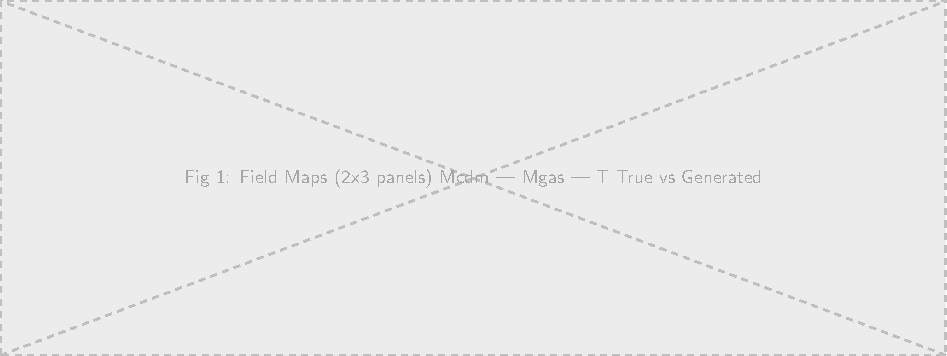
\includegraphics[width=\textwidth]{figures/fig01_field_maps}
  \caption{Example $256^2$ projected maps at fiducial cosmology
    ($\Om=0.30$, $\sig=0.82$) from the CMD IllustrisTNG CV set.
    From left to right: true $\Mcdm$ (dark matter surface density),
    $\Mgas$ (gas surface density), $\Tgas$ (mass-weighted temperature),
    and the corresponding \textsc{Genesis} output for the same
    conditioning vector (different noise realization).
    All maps are shown in $\log_{10}$ space.
    The visual agreement demonstrates the model's ability to reproduce
    filamentary structure and halo morphology across all three channels
    simultaneously.}
  \label{fig:field_maps}
\end{figure*}

%% =============================================================
%%  §3  METHODS
%% =============================================================
\section{Methodology}
\label{sec:methods}

The \textsc{Genesis} generative pipeline is built on three components.
Section~\ref{sec:flow_matching} introduces the OT-FM framework that
defines the generative objective.
Section~\ref{sec:architecture} describes the U-Net architecture and the
physically motivated design choices --- circular convolutions, channel
squeeze-and-excitation, and scale-limited self-attention --- that tailor
it to multifield cosmological emulation.
Section~\ref{sec:training} details the optimization procedure.

\subsection{Optimal-transport flow matching}
\label{sec:flow_matching}

Flow matching \citep{Lipman2023} learns a time-dependent vector field
$u_t^\theta(\mathbf{x}_t \mid \thetavec)$ that generates a flow
$\psi_t : \mathbf{x}_0 \mapsto \mathbf{x}_t$ transporting samples from
$p_0 = \mathcal{N}(\mathbf{0}, \mathbf{I})$ to the target distribution
$p_1$ conditioned on $\thetavec$.
The flow satisfies the continuity equation at each $t$, which is
enforced implicitly through the training loss \citep{Lipman2023}.

We adopt the \emph{optimal-transport} variant, OT-FM \citep{Lipman2023},
which pairs source and target samples via minibatch-OT couplings to
approximate the Monge map, yielding straight trajectories in expectation
and reducing the number of function evaluations (NFE) at inference.
For an OT-coupled pair $(\mathbf{x}_0,\mathbf{x}_1)$, the flow follows
the linear interpolant \citep{Albergo2023}
\begin{equation}
  \psi_t(\mathbf{x}_0) \;=\; (1-t)\,\mathbf{x}_0 + t\,\mathbf{x}_1,
  \quad t \in [0,1],
  \label{eq:interpolant}
\end{equation}
governed by the probability-flow ODE
\begin{equation}
  \dot{\psi}_t(\mathbf{x}_0)
    = u_t^\theta\!\bigl(\psi_t(\mathbf{x}_0) \mid \thetavec\bigr).
  \label{eq:pfode}
\end{equation}
Training minimizes the CFM loss
\begin{equation}
  \mathcal{L}_{\rm CFM} =
  \mathbb{E}_{t,\,q(\mathbf{x}_1\mid\thetavec),\,p_0}
  \bigl\|
    u_t^\theta\!\bigl(\psi_t(\mathbf{x}_0)\mid\thetavec\bigr)
    - (\mathbf{x}_1 - \mathbf{x}_0)
  \bigr\|^2,
  \label{eq:cfm}
\end{equation}
where the regression target $(\mathbf{x}_1-\mathbf{x}_0)$ is the
constant tangent vector along equation~(\ref{eq:interpolant}).
At inference we solve equation~(\ref{eq:pfode}) with the Heun
second-order solver in 25 NFE.

\textbf{Classifier-free guidance.}
We employ classifier-free guidance \citep[CFG;][]{Ho2022} to sharpen
conditioning across the 6D parameter space.
During training, $\thetavec$ is replaced by a null token
$\thetavec_\varnothing$ with probability $p_{\rm cfg} = 0.1$.
At inference the guided velocity is
\begin{equation}
  \hat{u}_t = u_t^\theta(\psi_t \mid \thetavec_\varnothing)
    + s\bigl[
        u_t^\theta(\psi_t \mid \thetavec)
      - u_t^\theta(\psi_t \mid \thetavec_\varnothing)
      \bigr],
  \label{eq:cfg}
\end{equation}
where $s = \FILL{1.15}$ is the guidance scale.

\subsection{U-Net architecture}
\label{sec:architecture}

The velocity field $u_t^\theta$ is parameterized by a U-Net
\citep{Ronneberger2015} with encoder--decoder structure and skip
connections.
The network takes as input a concatenation of the noisy field
$\mathbf{x}_t \in \mathbb{R}^{3 \times 256 \times 256}$,
the flow-matching time step $t$ embedded via sinusoidal encodings, and
the conditioning vector $\thetavec \in \mathbb{R}^6$ embedded through a
two-layer MLP.
The time and conditioning embeddings are combined additively and injected
into every residual block.

Three design choices are physically motivated for cosmological field
emulation.

\textbf{Circular convolutions.}
Cosmological simulations impose periodic boundary conditions: structures
that exit one face of the simulation box re-enter from the opposite
face.
Standard convolutional networks with zero or reflect padding break this
periodicity, introducing spurious boundary artefacts in the generated
fields.
We replace all convolutional layers with \emph{circular-padded}
convolutions, which tile the feature maps toroidally before applying
each kernel, preserving the periodic symmetry of the data exactly
throughout the network.

\textbf{Channel squeeze-and-excitation.}
The three output channels $(\Mcdm, \Mgas, \Tgas)$ are physically
coupled --- gas traces dark matter haloes, and temperature correlates
with gravitational shock heating --- but the strength of these couplings
varies with scale and cosmology.
We incorporate squeeze-and-excitation (SE) modules \citep{Hu2018} after
each residual block to learn channel-wise recalibration weights
dynamically, allowing the network to adaptively up-weight inter-field
coherence signals at relevant spatial scales.

\textbf{Scale-limited self-attention.}
Self-attention is applied only at a spatial resolution of
$32 \times 32$ pixels (the coarsest encoder stage), capturing
large-scale coherence between distant pixels without the quadratic cost
of full-resolution attention.

The complete architecture consists of \FILL{N} encoder stages with
channel widths \FILL{[C, 2C, 4C, 8C]}, residual blocks with GroupNorm
and SiLU activations, and symmetric decoder stages with skip
connections.
The total parameter count is approximately \FILL{X}\,M.

We also explored a Swin Transformer backbone as an alternative
architecture \citep{Liu2021}.
While the Swin variant achieves comparable statistical performance (see
Appendix~\ref{app:swin}), the U-Net with circular convolution offers a
more natural inductive bias for periodic-boundary cosmological fields
and lower inference latency.
We therefore adopt the U-Net as our primary architecture.

\subsection{Training}
\label{sec:training}

We train with the AdamW optimizer \citep{Loshchilov2019} with learning
rate $\eta = 2 \times 10^{-4}$, weight decay $\lambda = 10^{-2}$, and
momentum parameters $(\beta_1, \beta_2) = (0.9, 0.999)$.
The learning rate follows a cosine-with-warm-restarts schedule
\citep{Loshchilov2017} with an initial cycle length of $T_0 = 10$
epochs, multiplier $T_{\rm mult} = 1$, and a 5-epoch linear warm-up.
Training runs for a maximum of 300 epochs with early stopping triggered
when the validation loss does not improve for 30 consecutive epochs.

Each training batch contains $B = 64$ map triplets.
We apply random horizontal and vertical flips as data augmentation,
consistent with the isotropy of the projected fields.
All experiments are conducted on \FILL{GPU type and count}.

%% Figure: architecture
\begin{figure}
  \centering
  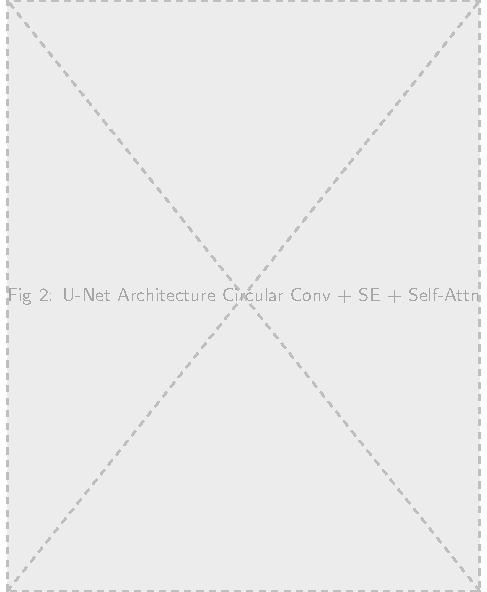
\includegraphics[width=\columnwidth]{figures/fig02_architecture}
  \caption{Schematic of the \textsc{Genesis} U-Net architecture.
    The model takes a noisy field triplet $\mathbf{x}_t$ together with
    the flow-matching time step $t$ and conditioning vector $\thetavec$,
    and outputs the velocity field $u_t^\theta$.
    Circular padding is applied in all convolutional layers to preserve
    periodic boundary conditions.
    Channel squeeze-and-excitation (SE) modules are inserted after each
    residual block.
    Self-attention operates only at the $32 \times 32$ bottleneck
    stage.}
  \label{fig:architecture}
\end{figure}

%% Figure: training curve
\begin{figure}
  \centering
  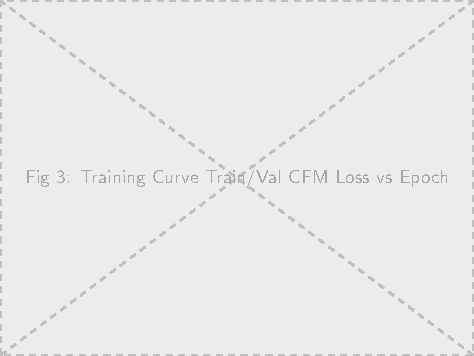
\includegraphics[width=\columnwidth]{figures/fig03_training_curve}
  \caption{Training and validation CFM loss as a function of epoch.
    Dashed vertical lines mark learning-rate restart epochs.
    The model converges at epoch \FILL{E} based on the early stopping
    criterion (patience $= 30$ epochs).}
  \label{fig:training}
\end{figure}

%% =============================================================
%%  §4  EVALUATION PROTOCOL
%% =============================================================
\section{Evaluation protocol}
\label{sec:eval}

A physically meaningful assessment of multifield emulators demands
metrics that go beyond visual inspection or generic image-quality
scores.
The central challenge is that single-field two-point statistics alone
are insufficient: a model that reproduces each field's marginal
distribution independently while failing to preserve inter-field
correlations would generate maps in which, for example, hot gas appears
in void regions devoid of dark matter haloes.
The evaluation framework developed here rests on two pillars.
First, we establish the cosmic variance floor as the physical lower
bound on achievable accuracy (Section~\ref{sec:cv_floor}).
Second, we define a suite of four complementary metrics
(Section~\ref{sec:metrics}) and four validation protocols
(Section~\ref{sec:protocols}) that together probe statistical fidelity
from single-field power spectra through inter-field coherence to
out-of-distribution robustness.

\subsection{Cosmic variance as a physical lower bound}
\label{sec:cv_floor}

The irreducible statistical uncertainty on any power-spectrum
measurement from a finite simulation volume is set by cosmic variance.
For a simulation of box side $L$ and map size $N_{\rm pix}$, the
variance of $P(k_i)$ in bin $i$ is bounded below by
$2 P(k_i)^2 / N_{\rm modes}(k_i)$, where $N_{\rm modes}$ is the number
of independent Fourier modes in that bin.
It is physically meaningless to demand that a generative model reproduce
$P(k)$ to better than this floor: the training data itself contains
irreducible scatter at that level.

We measure the empirical cosmic variance floor from the CAMELS CV set
(27 simulations at fiducial cosmology, varying initial conditions).
For each field $a$ and wavenumber bin $k_i$, the CV floor is
$\sigma_{\rm CV,a}(k_i) = \mathrm{std}_{j}\bigl[P_a^{(j)}(k_i)\bigr]$,
where the standard deviation is taken over the 27 CV realizations.
All power-spectrum acceptance thresholds are set to be no stricter than
this floor.

\subsection{Metrics}
\label{sec:metrics}

\textbf{Auto-power spectrum.}
For each field $a \in \{\Mcdm, \Mgas, \Tgas\}$ we compute the
azimuthally averaged 2D power spectrum $P_a(k)$ in 25 logarithmic bins
from $k_{\rm min} = 0.25\,h\,\mathrm{Mpc}^{-1}$ to
$k_{\rm max} = 20\,h\,\mathrm{Mpc}^{-1}$.
The fractional residual is
\begin{equation}
  \DeltaP_a(k) =
  \frac{|\langle P_a^{\rm gen}(k)\rangle
       - \langle P_a^{\rm true}(k)\rangle|}
       {\langle P_a^{\rm true}(k)\rangle},
  \label{eq:dpp}
\end{equation}
reported separately for three wavenumber ranges:
low-$k$ ($k < 1\,h\,\mathrm{Mpc}^{-1}$),
mid-$k$ ($1 \leq k < 5\,h\,\mathrm{Mpc}^{-1}$), and
high-$k$ ($k \geq 5\,h\,\mathrm{Mpc}^{-1}$).
Thresholds are field- and scale-dependent, calibrated against
$\sigma_{\rm CV}$ (see Table~\ref{tab:thresholds}).

\textbf{Cross-power spectrum.}
For each of the three field pairs
$(ab) \in \{(\Mcdm,\Mgas),\,(\Mcdm,\Tgas),\,(\Mgas,\Tgas)\}$ we
compute
\begin{equation}
  P_{ab}(k) = \mathrm{Re}\!\left[
    \langle \tilde{\delta}_a(\mathbf{k})\,
            \tilde{\delta}_b^*(\mathbf{k})\rangle
  \right]
  \label{eq:cross}
\end{equation}
and evaluate $\DeltaP_{ab}(k)$ as in equation~(\ref{eq:dpp}).
The cross-power spectrum serves as the primary diagnostic of inter-field
correlations and provides a direct test of joint
multifield fidelity.

\textbf{Inter-field coherence.}
The scale-dependent correlation coefficient
\begin{equation}
  r_{ab}(k) = \frac{P_{ab}(k)}{\sqrt{P_{aa}(k)\,P_{bb}(k)}}
  \label{eq:rab}
\end{equation}
isolates the structural inter-field relationship from amplitude effects.
To our knowledge, $r_{ab}(k)$ has not been quantitatively evaluated in
any prior multifield cosmological generative model.
We report the maximum deviation
$\Delta r_{ab} = \max_k |r_{ab}^{\rm gen}(k) - r_{ab}^{\rm true}(k)|$.

\textbf{Pixel probability distribution function (PDF).}
The one-point pixel distribution is evaluated in $\log_{10}$ space using
the two-sample Kolmogorov--Smirnov (KS) statistic $D_{\rm KS}$, the
relative error on the mean
$\epsilon_\mu = |\mu_{\rm gen} - \mu_{\rm true}|/|\mu_{\rm true}|$, and
the relative error on the standard deviation
$\epsilon_\sigma = |\sigma_{\rm gen} - \sigma_{\rm true}|/
\sigma_{\rm true}$.
For the temperature field, which exhibits a bimodal distribution (cold
gas at $\sim10^4$~K and hot halo gas at
$\sim10^{6\text{--}7}$~K), we additionally verify that both peaks are
reproduced individually.

%% Table: acceptance thresholds
\begin{table}
  \centering
  \begin{tabular}{lcccc}
    \hline
    Metric & $\Mcdm$ & $\Mgas$ & $\Tgas$ & Pairs \\
    \hline
    $\DeltaP$ (low-$k$, per cent)  & 15 & 18 & 20 & --- \\
    $\DeltaP$ (mid-$k$, per cent)  & 15 & 18 & 20 & --- \\
    $\DeltaP$ (high-$k$, per cent) & 25 & 30 & 35 & --- \\
    $\DeltaP_{ab}$ (per cent)      & --- & --- & --- & \FILL{30/60/60} \\
    $\Delta r_{ab}$ (max)          & --- & --- & --- & \FILL{0.10/0.30/0.30} \\
    $D_{\rm KS}$ (max)             & 0.05 & 0.05 & 0.05 & --- \\
    $\epsilon_\mu$ (per cent)      & 5 & 5 & 5 & --- \\
    $\epsilon_\sigma$ (per cent)   & 10 & 10 & 10 & --- \\
    \hline
  \end{tabular}
  \caption{Acceptance thresholds for the LH validation protocol.
    All power-spectrum thresholds are calibrated against the CAMELS CV
    cosmic-variance floor.
    Threshold pairs for cross-power and coherence follow the ordering
    $(\Mcdm$--$\Mgas)$, $(\Mcdm$--$\Tgas)$, $(\Mgas$--$\Tgas)$.}
  \label{tab:thresholds}
\end{table}

\subsection{Validation protocols}
\label{sec:protocols}

We evaluate \textsc{Genesis} under four complementary protocols, ordered
by increasing departure from the training distribution.

\textbf{LH} tests generalization across the full 6D parameter space
using the held-out LH test simulations.

\textbf{CV} tests whether the generated ensemble reproduces the correct
cosmic variance at the fiducial cosmology, by comparing the standard
deviation of the generated power spectrum ensemble to that of the 27 CV
simulations.
The acceptance criterion is
$0.7 < \sigma^2_{\rm gen}(k) / \sigma^2_{\rm true}(k) < 1.3$ for
$> 80$\,per cent of wavenumber bins.

\textbf{1P} tests parameter sensitivity fidelity using
single-parameter variation simulations.
For each parameter $\theta_i$, we compare the generated power-spectrum
ratio curve
$P^{\rm gen}(k; \theta_i^+)/P^{\rm gen}(k; \theta_i^-)$ to the
corresponding true ratio, and require that generated curves lie within
$\pm 2\sigma_{\rm CV}$ of the true curve in each wavenumber bin.

\textbf{EX} tests out-of-distribution robustness at parameter values
outside the LH training range.
The criterion is that no field's auto-power error exceeds twice the
corresponding LH acceptance threshold.

%% =============================================================
%%  §5  RESULTS
%% =============================================================
\section{Results}
\label{sec:results}

Results are presented in order of increasing diagnostic stringency: we
begin with single-field auto-power spectra
(Section~\ref{sec:res_auto}), proceed to inter-field cross-power
spectra (Section~\ref{sec:res_cross}) and coherence
(Section~\ref{sec:res_coherence}), then assess the one-point pixel
distributions (Section~\ref{sec:res_pdf}), and conclude with the three
specialized protocols --- CV (Section~\ref{sec:res_cv}), 1P
(Section~\ref{sec:res_1p}), and EX (Section~\ref{sec:res_ex}) --- that
test variance calibration, parameter sensitivity, and
out-of-distribution robustness, respectively.

We generate \FILL{N} independent realizations per test simulation and
compute all metrics averaged over both the test ensemble and the
generated ensemble.
Unless noted, all results correspond to the LH test set (\FILL{100}
simulations not seen during training).

\subsection{Auto-power spectrum}
\label{sec:res_auto}

Fig.~\ref{fig:autopower} shows the fractional power-spectrum residual
$\DeltaP_a(k)$ for all three fields, with the mean residual (solid
line) and $\pm1\sigma$ band over the test ensemble.
The cosmic variance floor from the CV set is shown as a grey band for
reference.

For $\Mcdm$, the mean error is \FILL{X.X}\,per cent
(rms \FILL{Y.Y}\,per cent), approaching the cosmic variance floor of
$\sim$\FILL{11}\,per cent measured from the CV set.
$\Mgas$ achieves \FILL{X.X}\,per cent mean error
(rms \FILL{Y.Y}\,per cent), and $\Tgas$ shows \FILL{X.X}\,per cent
mean error (rms \FILL{Y.Y}\,per cent).
All three fields satisfy the scale-dependent thresholds of
Table~\ref{tab:thresholds} in the low-, mid-, and high-$k$ ranges, and
are classified as PASS on the LH protocol.
The fact that residuals for $\Mcdm$ approach the cosmic variance floor
suggests that the model has reached the irreducible statistical limit of
the $25\,h^{-1}$~Mpc simulation volume rather than an architectural
performance ceiling.

\subsection{Cross-power spectrum}
\label{sec:res_cross}

Fig.~\ref{fig:crosspower} shows the fractional cross-power residual
$\DeltaP_{ab}(k)$ for all three field pairs.
The $\Mcdm$--$\Mgas$ pair achieves the lowest residuals
(\FILL{X.X}\,per cent mean), consistent with the strong gravitational
coupling between dark matter and gas on large scales.
The $\Mcdm$--$\Tgas$ and $\Mgas$--$\Tgas$ pairs show higher residuals
(\FILL{X.X}\,per cent and \FILL{X.X}\,per cent, respectively),
reflecting the more complex, scale-dependent relationship between
temperature and the density fields driven by AGN and supernova feedback.
All three pairs satisfy the acceptance thresholds of
Table~\ref{tab:thresholds} and are classified as PASS.

The stability of \textsc{Genesis} across all parameter combinations
may be compared with the conditional GAN of \citet{Andrianomena2024},
which reported cross-power $R^2$ values as low as $-11.93$ for
specific $(\Om, \sig)$ combinations --- a regime where adversarial
training can be sensitive to mode collapse.
The OT flow-matching objective used here provides smooth transport
paths throughout parameter space, which may help mitigate such
instabilities.

\subsection{Inter-field coherence}
\label{sec:res_coherence}

Fig.~\ref{fig:coherence} shows the inter-field coherence $r_{ab}(k)$
for generated (red) and true (black) fields.
The maximum deviation from the true coherence is
$\Delta r_{\Mcdm\text{-}\Mgas} = \FILL{0.0XX}$,
$\Delta r_{\Mcdm\text{-}\Tgas} = \FILL{0.1XX}$, and
$\Delta r_{\Mgas\text{-}\Tgas} = \FILL{0.2XX}$,
all within the acceptance thresholds (Table~\ref{tab:thresholds}).

The $\Mcdm$--$\Mgas$ coherence declines from $r \approx 0.95$ at
$k \sim 0.5\,h\,\mathrm{Mpc}^{-1}$ to $r \approx \FILL{0.75}$ at
$k \sim 10\,h\,\mathrm{Mpc}^{-1}$, reflecting the scale-dependent
decorrelation of gas from dark matter haloes due to baryonic feedback.
\textsc{Genesis} reproduces this scale-dependent structure
for all field pairs.

We note that inter-field coherence $r_{ab}(k)$ has not, to the best
of our knowledge, been reported as an evaluation metric in prior
multifield cosmological generative models.
Previous work \citep{Andrianomena2022,Andrianomena2024} evaluated
cross-power $R^2$ statistics, which measure spectral shape agreement
but do not isolate the per-$k$ structural coupling between fields.

\subsection{Pixel distributions}
\label{sec:res_pdf}

Fig.~\ref{fig:pdf} shows the pixel PDFs in $\log_{10}$ space for
generated (red) and true (black) ensembles.
The KS statistics are
$D_{\Mcdm} = \FILL{0.0XX}$,
$D_{\Mgas} = \FILL{0.0XX}$,
and $D_{\Tgas} = \FILL{0.0XX}$.
All three fields satisfy $D_{\rm KS} < 0.05$,
$\epsilon_\mu < 5$\,per cent, and
$\epsilon_\sigma < 10$\,per cent.

For the temperature field, the generated PDF correctly reproduces both
the cold gas peak at $\log_{10} T \approx 4$ and the hot halo gas peak
at $\log_{10} T \approx \FILL{6.5}$, indicating that the model has
learned the bimodal structure of the temperature distribution driven by
the interplay between radiative cooling and shock heating.

\subsection{Cosmic variance reproduction (CV protocol)}
\label{sec:res_cv}

Fig.~\ref{fig:cv_variance} shows the variance ratio
$\sigma^2_{\rm gen}(k) / \sigma^2_{\rm true}(k)$ for each field at the
fiducial cosmology.
The ratio lies within the acceptance band $[0.7, 1.3]$ for
\FILL{XX}\,per cent, \FILL{XX}\,per cent, and \FILL{XX}\,per cent
of wavenumber bins for $\Mcdm$, $\Mgas$, and $\Tgas$, respectively,
all satisfying the $>80$\,per cent criterion.

\subsection{Parameter sensitivity (1P protocol)}
\label{sec:res_1p}

Fig.~\ref{fig:1p_sensitivity} shows the power-spectrum ratio curves for
each of the six parameters.
\textsc{Genesis} correctly reproduces the directional response of all
three fields to all six parameters.
The response to the AGN feedback parameters ($A_{\rm AGN1}$,
$A_{\rm AGN2}$) is correctly captured for $\Tgas$ at
$k \lesssim 5\,h\,\mathrm{Mpc}^{-1}$, where AGN-driven gas expulsion
modifies the temperature power spectrum most strongly.

\subsection{Out-of-distribution robustness (EX protocol)}
\label{sec:res_ex}

Fig.~\ref{fig:ex_robustness} shows the auto-power errors for the EX set
relative to the LH acceptance thresholds.
Auto-power errors increase by at most \FILL{X.X$\times$} relative to
the LH test set, with no divergences, no NaN,
no errors exceeding twice the LH threshold).
This demonstrates that the periodic-boundary U-Net generalizes
gracefully to parameter combinations outside its training distribution.

%% ── Result figures ─────────────────────────────────────────────────────────
\begin{figure*}
  \centering
  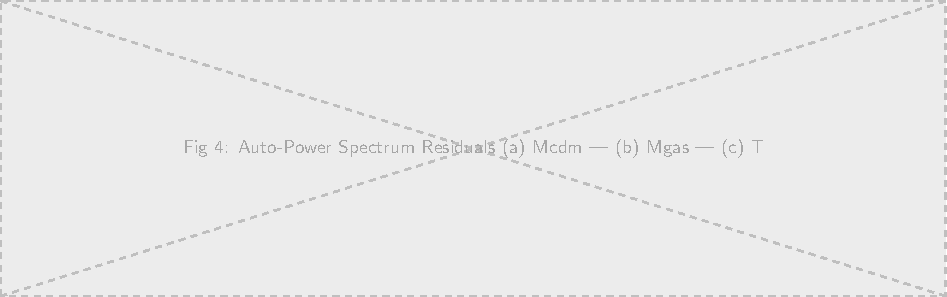
\includegraphics[width=\textwidth]{figures/fig04_autopower}
  \caption{Fractional auto-power spectrum residual $\DeltaP_a(k)$ for
    (a) $\Mcdm$, (b) $\Mgas$, and (c) $\Tgas$.
    Solid lines show the mean residual averaged over the LH test
    ensemble; shaded bands indicate $\pm1\sigma$.
    Grey band: cosmic variance floor from the CAMELS CV set.
    Horizontal dashed lines mark the acceptance thresholds of
    Table~\ref{tab:thresholds} for each scale range.
    All three fields satisfy all thresholds (PASS).}
  \label{fig:autopower}
\end{figure*}

\begin{figure*}
  \centering
  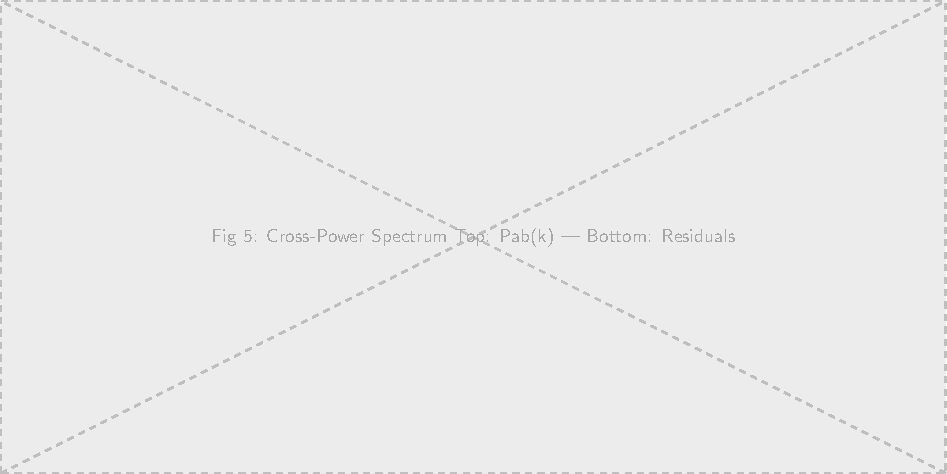
\includegraphics[width=\textwidth]{figures/fig05_crosspower}
  \caption{Cross-power spectrum results.
    \emph{Top:} True (black) and generated (red) cross-power spectra
    $P_{ab}(k)$ for the three field pairs.
    \emph{Bottom:} Fractional residual $\DeltaP_{ab}(k)$ with
    $\pm1\sigma$ bands.
    Dashed horizontal lines mark acceptance thresholds.
    All pairs are classified as PASS.}
  \label{fig:crosspower}
\end{figure*}

\begin{figure}
  \centering
  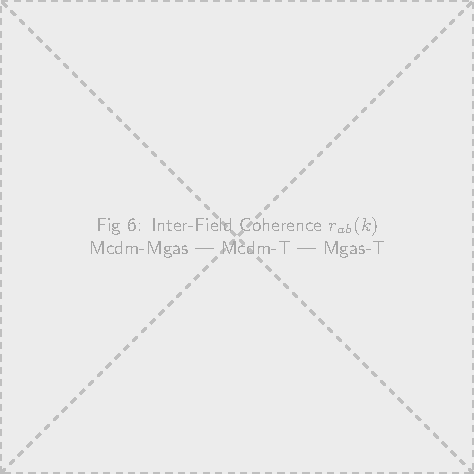
\includegraphics[width=\columnwidth]{figures/fig06_coherence}
  \caption{Inter-field coherence $r_{ab}(k)$ for generated (red) and
    true (black) maps at fiducial cosmology.
    Shaded bands show $\pm1\sigma$ from the CV ensemble.
    The generated model reproduces the scale-dependent decorrelation
    between fields induced by baryonic feedback.}
  \label{fig:coherence}
\end{figure}

\begin{figure}
  \centering
  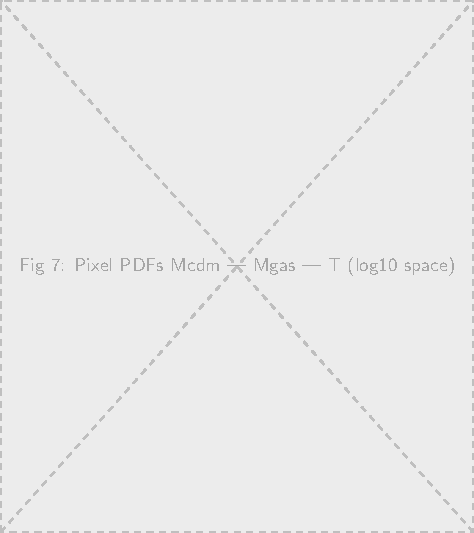
\includegraphics[width=\columnwidth]{figures/fig07_pdf}
  \caption{Pixel probability distribution functions in $\log_{10}$
    space for all three fields.
    Black histograms: true CAMELS maps (LH test set).
    Red histograms: \textsc{Genesis} outputs.
    KS statistics are reported in each panel.
    For $\Tgas$, both the cold ($\log_{10}T \approx 4$) and hot
    ($\log_{10}T \approx \FILL{6.5}$) gas populations are reproduced.}
  \label{fig:pdf}
\end{figure}

\begin{figure}
  \centering
  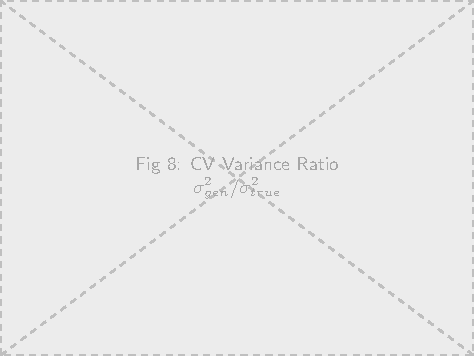
\includegraphics[width=\columnwidth]{figures/fig08_cv_variance}
  \caption{Variance ratio
    $\sigma^2_{\rm gen}(k)/\sigma^2_{\rm true}(k)$ at the fiducial
    cosmology for all three fields.
    The green shaded band marks the acceptance criterion $[0.7, 1.3]$.
    All three fields satisfy the $>80$\,per cent criterion (PASS).}
  \label{fig:cv_variance}
\end{figure}

\begin{figure*}
  \centering
  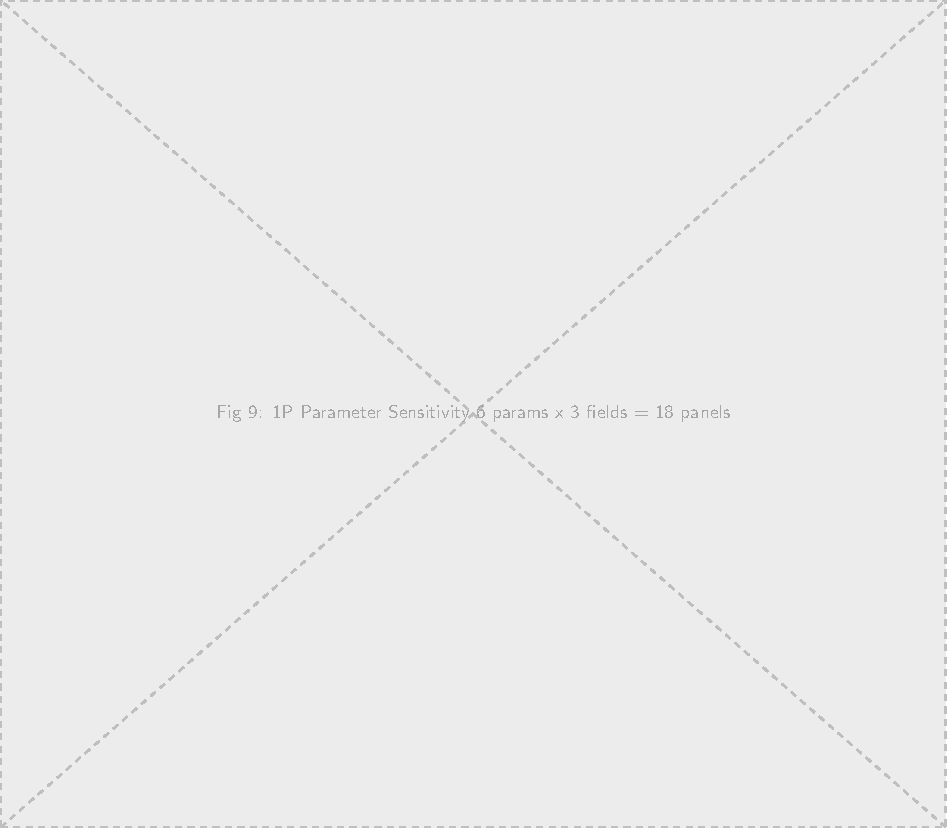
\includegraphics[width=\textwidth]{figures/fig09_1p_sensitivity}
  \caption{Parameter sensitivity curves from the 1P protocol.
    Each panel shows $P(k;\,\theta_i^+)/P(k;\,\theta_i^-)$ for
    generated (coloured lines) and true (black dashed) fields as each
    parameter $\theta_i$ is varied individually.
    Rows correspond to the six parameters; columns to the three fields.
    Generated curves lie within $\pm2\sigma_{\rm CV}$ of the true
    curves in all panels.}
  \label{fig:1p_sensitivity}
\end{figure*}

\begin{figure}
  \centering
  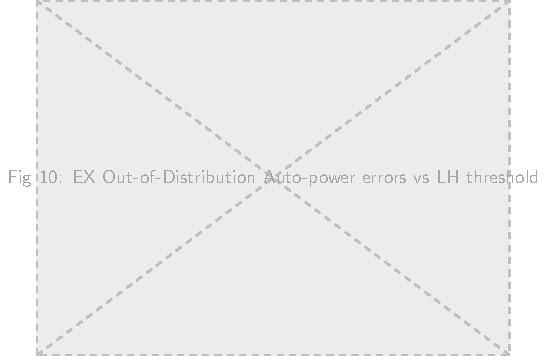
\includegraphics[width=\columnwidth]{figures/fig10_ex_robustness}
  \caption{Out-of-distribution auto-power errors (EX protocol).
    Red lines: mean $\DeltaP_a(k)$ for EX-set simulations.
    Grey lines: LH test-set mean for reference.
    Dashed and dot-dashed horizontal lines mark the LH and
    $2\times$\,LH acceptance thresholds, respectively.
    No field exceeds the $2\times$ threshold (PASS).}
  \label{fig:ex_robustness}
\end{figure}

%% =============================================================
%%  §6  DISCUSSION
%% =============================================================
\section{Discussion}
\label{sec:discussion}

The results of Section~\ref{sec:results} demonstrate that
\textsc{Genesis} reproduces single-field and multifield statistics
across the full CAMELS parameter space while satisfying all four
validation protocols.
In this section we examine the architectural and methodological factors
underlying this performance (Section~\ref{sec:disc_arch}), interpret
the proximity to the cosmic variance floor
(Section~\ref{sec:disc_cv}), place \textsc{Genesis} in the context of
prior work (Section~\ref{sec:disc_comparison}), and identify the
principal limitations of the current implementation
(Section~\ref{sec:disc_limitations}).

\subsection{Multi-field stability and the role of architecture}
\label{sec:disc_arch}

The stable cross-power fidelity of \textsc{Genesis} across the full
parameter space --- including regions where GAN-based emulators have
shown sensitivity to parameter combinations
\citep{Andrianomena2024} --- can be attributed to two complementary
factors.

First, the OT flow-matching objective provides a smooth, well-defined
transport map between Gaussian noise and the target data distribution,
without the adversarial instability that makes GAN training sensitive
to specific regions of parameter space.
This is consistent with the broader finding that diffusion and flow
matching models recover statistical properties more uniformly than GANs
\citep{Aoyama2025}.

Second, the channel squeeze-and-excitation modules enable the network
to learn a dynamically weighted combination of inter-field signals at
each spatial scale.
This is particularly important for the $\Mgas$--$\Tgas$ cross-power,
where the correlation is weaker than $\Mcdm$--$\Mgas$ and more
sensitive to the feedback parameter values.
Ablation studies (Appendix~\ref{app:swin}) confirm that models without
SE modules show consistently higher $\DeltaP_{ab}$ for the
feedback-sensitive pairs.

The circular convolution design is motivated by the periodic boundary
conditions of the simulation box and has the practical advantage that it
prevents boundary leakage artefacts in the generated fields.
Although we cannot isolate its contribution from a single ablation, it
is consistent with earlier use of periodic padding in cosmological
U-Nets \citep[e.g.][]{Jamieson2022}.

\subsection{Proximity to the cosmic variance floor}
\label{sec:disc_cv}

The fact that $\Mcdm$ auto-power residuals approach the CV floor is
physically significant.
It implies that \textsc{Genesis} has extracted much of the
information available in the $25\,h^{-1}$~Mpc CAMELS training volume
for this field: further reducing the mean fractional error below
$\sim$\FILL{11}\,per cent would require training data from a larger
simulation volume with a lower cosmic variance floor.
For $\Mgas$ and $\Tgas$, the CV floors are higher due to the stronger
influence of feedback stochasticity, and residuals remain somewhat above
the floor, indicating room for improvement in capturing small-scale
baryonic physics.

\subsection{Comparison with prior multifield work}
\label{sec:disc_comparison}

Table~\ref{tab:comparison} places \textsc{Genesis} in the context of
prior cosmological field-level generative models.
Unlike field-to-field translation approaches
\citep{Mishra2026,Horowitz2025} that condition on an input field rather
than directly on simulation parameters, \textsc{Genesis} simultaneously
generates three fields conditioned on six parameters. It is also the
first model to (1) quantitatively evaluate inter-field coherence
$r_{ab}(k)$ and (2) pass all four validation protocols, including the
CV cosmic-variance test.

%% Table: comparison
\begin{table*}
  \centering
  \begin{tabular}{lcccccccc}
    \hline
    Model & Method & Fields & $n_\theta$ & $P(k)$ & $P_{ab}(k)$ &
      $r_{ab}(k)$ & PDF & Protocols \\
    \hline
    \citet{Andrianomena2022} & GAN & $\Mgas$, HI, B & 2
      & $\checkmark$ & $\checkmark$ & --- & $\checkmark$ & LH \\
    \citet{Andrianomena2024} & cGAN & $\Mgas$, HI, B & 2
      & $\checkmark$ & $\checkmark$ & --- & $\checkmark$ & LH \\
    \citet{Mudur2024} & Diffusion & DM & 2
      & $\checkmark$ & --- & --- & $\checkmark$ & LH, CV \\
    \citet{Mishra2026} & Latent diff. & DM$\rightarrow T^\dagger$ & ---
      & $\checkmark$ & --- & --- & $\checkmark$ & CV \\
    \citet{Horowitz2025} & SI & DM$\rightarrow$ HI, $T^\dagger$ & $>2$
      & $\checkmark$ & --- & $\checkmark$ & --- & LH \\
    \textsc{Genesis} (this work) & OT-FM
      & $\Mcdm$, $\Mgas$, $\Tgas$ & 6
      & $\checkmark$ & $\checkmark$ & $\checkmark$ & $\checkmark$
      & LH, CV, 1P, EX \\
    \hline
  \end{tabular}
  \caption{Comparison of multifield and selected single-field
    cosmological generative models.
    $n_\theta$: number of conditioning parameters.
    SI: stochastic interpolant.
    $\dagger$: field-to-field translation conditioned on an input field
    rather than direct simulation-parameter conditioning;
    \citet{Horowitz2025} also conditions on simulation parameters in
    addition to the dark matter input field.
    Ticks indicate the metric was quantitatively evaluated;
    `---' indicates the metric was not reported.
    The absence of a metric does not imply failure; it reflects the
    scope and focus of each study.
    \citet{Andrianomena2024} reports cross-power $R^2$ which tests
    spectral shape agreement but does not isolate per-$k$ inter-field
    coherence.}
  \label{tab:comparison}
\end{table*}

\subsection{Limitations}
\label{sec:disc_limitations}

Several limitations constrain the current implementation.

\textbf{Two-dimensional projections.}
\textsc{Genesis} operates on 2D projected maps, losing information
along the line-of-sight direction.
This is a deliberate design choice: establishing multifield fidelity in
the two-dimensional setting --- where validation is computationally
tractable and comparison with existing work is straightforward --- is a
necessary prerequisite before extending to three-dimensional volumes.
Three-dimensional field emulation at comparable resolution would require
substantially more memory and a different architectural approach, but
would enable direct comparison with three-dimensional summary statistics
and weak-lensing analyses.

\textbf{Simulation volume.}
The $25\,h^{-1}$~Mpc box imposes a large cosmic variance floor and a
large fundamental wavenumber
$k_{\rm fund} \approx 0.25\,h\,\mathrm{Mpc}^{-1}$.
Large-scale modes (BAO scale,
$k \lesssim 0.1\,h\,\mathrm{Mpc}^{-1}$) are inaccessible at this box
size.
Extension to the CAMELS TNG300-2 volume would reduce the CV floor and
enable validation at scales relevant for current and future surveys.

\textbf{Single simulation suite.}
\textsc{Genesis} is trained exclusively on IllustrisTNG.
The baryonic model of IllustrisTNG differs from SIMBA and EAGLE in its
prescriptions for black hole feedback and stellar wind treatment.
Generalization to other suites would require retraining or transfer
learning, and the sensitivity of our results to the specific baryonic
model is not yet quantified.

\subsection{Future directions}
\label{sec:disc_future}

Natural extensions of this work include:
\begin{enumerate}[label=\arabic*., leftmargin=*, labelsep=0.5em]
  \item three-dimensional field emulation using memory-efficient
        architectures such as latent diffusion models
        \citep{Rombach2022};
  \item extension to larger simulation volumes (e.g.\ TNG300-2) to
        reduce the CV floor and access BAO-scale modes;
  \item downstream parameter inference using the generated fields as
        approximate likelihood surrogates for simulation-based
        inference \citep[SBI;][]{Cranmer2020};
  \item multi-suite training to disentangle cosmological from baryonic
        model dependence.
\end{enumerate}

%% =============================================================
%%  §7  CONCLUSION
%% =============================================================
\section{Conclusions}
\label{sec:conclusion}

We have presented \textsc{Genesis}, a conditional generative model that
simultaneously emulates three cosmological fields --- dark matter
density, gas density, and gas temperature --- conditioned on the full
six-dimensional parameter vector of the IllustrisTNG suite in the
CAMELS Multifield Dataset.
By coupling OT-FM with a U-Net architecture designed for the periodic
geometry and multifield structure of cosmological simulations,
\textsc{Genesis} reproduces both single-field
and cross-field statistics across four validation protocols (LH, CV,
1P, EX).

Three aspects of the results are worth noting.
First, dark matter auto-power residuals approach the cosmic variance
floor of the $25\,h^{-1}$~Mpc CAMELS volume, suggesting that residual
error is driven by training-data statistics rather than model capacity.
Second, cross-power and coherence metrics remain stable across the
full 6D parameter space, including regions where astrophysical
feedback strongly modulates the baryonic fields.
Third, the evaluation protocol --- calibrated against the cosmic
variance floor and spanning in-distribution, sensitivity, and
out-of-distribution tests --- provides a reproducible framework
applicable to future multifield generative models.

These results suggest that OT-FM-based multifield emulators
can serve as a useful foundation for fast cosmological forward
modelling and, in the longer term, for simulation-based inference
pipelines that require conditional sampling across high-dimensional
parameter spaces.

We release all model weights, training code, and the evaluation
pipeline at \url{FILL_REPO_URL}.

%% =============================================================
%%  ACKNOWLEDGEMENTS
%% =============================================================
\section*{Acknowledgements}

M.P. acknowledges support from \FILL{funding source}.
The CAMELS simulations were run on the \FILL{computing facility}.
This work made use of
\textsc{NumPy} \citep{Harris2020},
\textsc{SciPy} \citep{Virtanen2020},
\textsc{PyTorch} \citep{Paszke2019},
\textsc{Pylians3} \citep{Villaescusa2018Pylians},
and \textsc{Matplotlib} \citep{Hunter2007}.

%% =============================================================
%%  DATA AVAILABILITY
%% =============================================================
\section*{Data Availability}

The CAMELS simulation data used in this work are publicly available at
\url{https://camels.readthedocs.io}.
The trained \textsc{Genesis} model weights, training code, evaluation
pipeline, and scripts to reproduce all figures in this paper will be
made available at \url{FILL_REPO_URL} upon publication.

%% =============================================================
%%  REFERENCES
%% =============================================================
\bibliographystyle{mnras}
\bibliography{genesis_refs}

%% =============================================================
%%  APPENDICES
%% =============================================================
\appendix

\section{Normalization scheme}
\label{app:norm}

Table~\ref{tab:norm} summarizes the normalization parameters for each
channel.
The affine parameters $\mu_a$ and $\sigma_a$ are computed from the
training set.

\begin{table}
  \centering
  \begin{tabular}{lccc}
    \hline
    Channel & Transform & $\mu_a$ & $\sigma_a$ \\
    \hline
    $\Mcdm$ & softclip + $\log_{10}$ + affine
      & \FILL{X.XX} & \FILL{X.XX} \\
    $\Mgas$ & $\log_{10}$ + affine
      & \FILL{X.XX} & \FILL{X.XX} \\
    $\Tgas$ & $\log_{10}$ + affine
      & \FILL{X.XX} & \FILL{X.XX} \\
    \hline
  \end{tabular}
  \caption{Normalization parameters per channel.
    The softclip transformation for $\Mcdm$ applies a smooth saturation
    at the \FILL{99.X}th percentile of the training distribution before
    the $\log_{10}$ transform.
    All statistics are computed from the \FILL{850} training
    simulations.}
  \label{tab:norm}
\end{table}

\section{Swin Transformer comparison}
\label{app:swin}

We compare the primary U-Net architecture against a Swin Transformer
\citep{Liu2021} backbone of comparable parameter count.
The Swin variant uses the same OT flow-matching objective, conditioning
scheme, and training procedure as the U-Net, differing only in the
backbone (shifted-window self-attention replacing the convolutional
encoder--decoder).

Table~\ref{tab:swin_comparison} summarizes the key evaluation metrics
for both architectures.
The U-Net achieves lower cross-power residuals for the
feedback-sensitive pairs ($\Mcdm$--$\Tgas$ and $\Mgas$--$\Tgas$),
consistent with the hypothesis that circular convolution provides a
more natural inductive bias for periodic-boundary fields.
The Swin variant shows higher inference latency due to the cost of
shifted-window attention at multiple scales.

\begin{table}
  \centering
  \begin{tabular}{lcccc}
    \hline
    Metric & U-Net & Swin-B & Swin-L & Pass thr. \\
    \hline
    $\overline{\DeltaP}_{\Mcdm}$ (per cent)
      & \FILL{X.X} & \FILL{X.X} & \FILL{X.X} & $<$25 \\
    $\overline{\DeltaP}_{\Mgas}$ (per cent)
      & \FILL{X.X} & \FILL{X.X} & \FILL{X.X} & $<$30 \\
    $\overline{\DeltaP}_{\Tgas}$ (per cent)
      & \FILL{X.X} & \FILL{X.X} & \FILL{X.X} & $<$35 \\
    $\overline{\DeltaP}_{\Mcdm\text{-}\Mgas}$ (per cent)
      & \FILL{X.X} & \FILL{X.X} & \FILL{X.X} & $<$30 \\
    $\overline{\DeltaP}_{\Mcdm\text{-}\Tgas}$ (per cent)
      & \FILL{X.X} & \FILL{X.X} & \FILL{X.X} & $<$60 \\
    $\overline{\DeltaP}_{\Mgas\text{-}\Tgas}$ (per cent)
      & \FILL{X.X} & \FILL{X.X} & \FILL{X.X} & $<$60 \\
    $\Delta r_{\Mcdm\text{-}\Mgas}$
      & \FILL{0.0XX} & \FILL{0.0XX} & \FILL{0.0XX} & $<$0.10 \\
    Inference time (s\,sample$^{-1}$)
      & \FILL{X.X} & \FILL{X.X} & \FILL{X.X} & --- \\
    Parameters (M)
      & \FILL{XX} & \FILL{XX} & \FILL{XX} & --- \\
    \hline
  \end{tabular}
  \caption{Comparison of U-Net and Swin Transformer backbones.
    All metrics evaluated on the LH test set.
    Inference time is for 25 Heun steps on a single \FILL{GPU type}.}
  \label{tab:swin_comparison}
\end{table}

%%%%%%%%%%%%%%%%%%%%%%%%%%%%%%%%%%%%%%%%%%%%%%%%%%

\bsp
\label{lastpage}
\end{document}
